\documentclass[10pt,letterpaper]{article}
\usepackage[T1]{fontenc}
\usepackage[utf8]{inputenc}
\usepackage{lmodern,amsmath,amssymb,amsthm,mathtools}
\usepackage{booktabs,microtype,geometry,graphicx,tikz}
\usepackage{algorithm,algpseudocode}
\usepackage[round,authoryear]{natbib}
\usepackage{xcolor}
\usepackage[colorlinks=true,linkcolor=blue!55!black,citecolor=blue!55!black,urlcolor=blue!55!black]{hyperref}
\usepackage[capitalise,noabbrev]{cleveref}
\geometry{margin=0.84in}
\setlength{\parskip}{0.20em}
\setlength{\parindent}{1.1em}
\newtheorem{proposition}{Proposition}
\newtheorem{lemma}{Lemma}
\newtheorem{remark}{Remark}
\newcommand{\RR}{\mathbb R}
\newcommand{\Ccut}{\mathcal C}
\newcommand{\one}{\mathbf 1}
\title{\bfseries Event-Driven Great-Semicircle Search for Objective-Guided Max-Cut Rounding}
\author{Heriberto Espino-Montelongo\\\small Universidad de las Am\'ericas Puebla}
\date{Research draft: November 2026\\\small Provisional empirical results; independent archive audit pending}
\begin{document}
\maketitle
\begin{abstract}
This paper studies direct optimization of hyperplane rounding for weighted and signed Max-Cut. Given a frozen semidefinite-programming (SDP) vector factor, we rotate a normal along a great semicircle and enumerate the finite sequence of vertex-crossing events. Signed cut gains update the objective between events, yielding an exact best cut along the selected arc in \(O(np+m+n\log n)\) time, for \(n\) vertices, \(m\) edges, and factor dimension \(p\), under exact arithmetic and sparse graph access. Repeated searches use random, gain-guided and boundary-guided tangents while retaining the initial Goemans--Williamson (GW) cut. We formulate the guarantee and its limits and document implementation-level semantics. A preliminary Experiment025 aggregate comparison on 71 G-set graphs, 18 methods, and 16 shared GW starts per graph and method reports a \(0.3176\%\) equal-graph mean best-of-16 improvement over identically refined GW (95\% graph-bootstrap interval \(0.2252\)--\(0.4196\%\); 59 wins, 7 ties, 5 losses). Results describe full initializer plus Flip/KL/ILS pipelines, not pure sweeping; independently rescored partitions, complete paired-seed records and equal-compute comparisons are pending. We distinguish established improved-rounding ideas from the particular finite-event search studied here.
\end{abstract}
\noindent\textbf{Keywords:} Max-Cut; semidefinite programming; event-driven line search; hyperplane rounding; signed graphs.

\section{Introduction}
The semidefinite relaxation of Max-Cut and random-hyperplane rounding \citep{goemans1995} give a strong baseline, but a single random hyperplane may miss better cuts realizable by the same vector embedding. Improved rounding is already a broad research area, encompassing outward rotations \citep{zwick1999,feige2006}, swept thresholds \citep{lang2004}, clustering \citep{rodriguez2020}, repeated SDP-based rounding \citep{felzenszwalb2022} and learned normal selection \citep{maliakal2025}. We therefore do not claim novelty for the generic idea of selecting a better hyperplane.

Our focus is a specific objective-aware mechanism: instead of evaluating arbitrary continuously rotated normals, sort the exact angles at which any embedded vertex changes sign. A single great-semicircle search is globally optimal \emph{within that rotation path}; repeatedly selecting paths is a heuristic over the sphere of normal directions. We give algorithmic details, formal proofs, signed-edge safeguards, and source-grounded preliminary empirical evidence.

\section{Signed Max-Cut and the fixed embedding}
Let \(G=(V,E,w)\) be an undirected weighted graph, \(|V|=n\), \(|E|=m\), no self-loops, and \(w_{ij}\in\RR\). For spins \(x\in\{-1,+1\}^n\), define
\begin{equation}\label{eq:cut}
\Ccut(x)=\sum_{\{i,j\}\in E}w_{ij}\one[x_i\ne x_j]
=\frac12\sum_{\{i,j\}\in E}w_{ij}(1-x_ix_j).
\end{equation}
The classical relaxation optimizes
\begin{equation}\label{eq:sdp}
\max_{X\succeq0,\ X_{ii}=1}\frac12\sum_{\{i,j\}\in E}w_{ij}(1-X_{ij}).
\end{equation}
Let \(Y\in\RR^{n\times p}\) be a \emph{fixed} SDP-derived factor, with rows \(y_i^\top\), where \(YY^\top=X\). The method never changes \(Y\) or resolves the SDP. For each unit normal \(r\in S^{p-1}\), its rounded labels and score are
\begin{equation}\label{eq:round}
x_i(r)=\begin{cases}+1,&y_i^\top r>0\\-1,&y_i^\top r\le0,\end{cases}
\qquad F(r)=\Ccut(x(r)).
\end{equation}
Different normals may induce the same partition. The search is restricted to partitions realizable by homogeneous separating hyperplanes of the fixed rows \(y_i\), whereas later discrete local search has no such restriction.

\section{One exact great-semicircle search}
Take unit \(r,u\in\RR^p\) with \(r^\top u=0\), and define
\begin{equation}\label{eq:arc}
r(\theta)=\cos\theta\,r+\sin\theta\,u,\qquad -\pi/2<\theta<\pi/2.
\end{equation}
The normal remains unit length. With \(a_i=y_i^\top r\) and \(b_i=y_i^\top u\), the projected coordinate is
\(q_i(\theta)=a_i\cos\theta+b_i\sin\theta\).
\begin{lemma}[Crossing angles]\label{lem:roots}
If \(b_i\ne0\), vertex \(i\) changes label exactly once in the open interval, at \(\theta_i=\arctan(-a_i/b_i)\). If \(b_i=0\) and \(a_i\ne0\), its sign is fixed. If \(a_i=b_i=0\), its projection vanishes throughout the path.
\end{lemma}
\begin{proof}
Since \(\cos\theta>0\) in the open interval, \(q_i(\theta)=0\) is equivalent to \(a_i+b_i\tan\theta=0\). The tangent is one-to-one and onto \(\RR\) there. The degenerate cases follow directly.
\end{proof}
Every interval between consecutive event angles induces a constant partition and constant cut value. Choosing the angular midpoint is merely a numerically convenient way to reconstruct one normal inside the winning interval; this is not a midpoint between SDP vectors.

For a partition \(x\), the signed gain of flipping vertex \(i\) is
\begin{equation}\label{eq:gain}
\Delta_i=\Ccut(x^{\oplus i})-\Ccut(x)
=x_i\sum_{j:\{i,j\}\in E}w_{ij}x_j.
\end{equation}
After that flip, its own gain changes sign and the gain of each neighbor \(j\) is updated by
\begin{equation}\label{eq:update}
\Delta_j\gets\Delta_j-2w_{ij}x_ix_j,
\end{equation}
using the spins immediately before the flip. These identities hold for signed weights. If several roots coincide, all corresponding vertices must flip before a cut value is considered for the next open interval.

\begin{proposition}[Exact fixed-arc search]\label{prop:exact}
Under exact arithmetic and a consistent treatment of vertices identically tied on the arc, sorting and scanning all crossing-event groups with \eqref{eq:gain}--\eqref{eq:update} finds the maximum signed cut over all open intervals of the given semicircle. The time is \(O(m+n\log n)\) after projections and sparse adjacency are available, hence \(O(np+m+n\log n)\) including dense factor projections.
\end{proposition}
\begin{proof}
By \cref{lem:roots} no vertex changes label except at a crossing event, so the cut is constant on each open interval. Initialize the cut immediately after the left endpoint and process event groups in sorted order. Each flip is accounted for exactly by \eqref{eq:gain}; \eqref{eq:update} maintains gains inductively. Thus every distinct interval cut is visited and the maximum recorded. Sorting needs \(O(n\log n)\); each vertex flips at most once and each edge participates in a constant number of gain updates. The two dense projections cost \(O(np)\).
\end{proof}
The actual code reconstructs a midpoint normal, independently rescales its cut on the original signed edges, and rejects an inconsistent predicted gain or a worsened realized cut. Floating-point root collisions can therefore cause a fallback rather than an exact arithmetic optimum.

\begin{algorithm}[t]
\caption{Exact signed sweep on a specified great semicircle}
\label{alg:arc}
\begin{algorithmic}[1]
\Require Signed graph \(G\); fixed factor \(Y\); unit normal \(r\) and tangent \(u\perp r\)
\State Compute \(a=Yr,b=Yu\); initialize signs at \(\theta\to-\pi/2^+\)
\State Initialize signed cut and gains; compute roots \(\arctan(-a_i/b_i)\) for \(b_i\ne0\)
\State Sort crossing events and record initial cut as best
\For{each group of equal-angle events in increasing order}
 \For{each crossing vertex \(i\) in the group}
   \State Update cut by \(\Delta_i\); update neighboring gains; flip \(i\)
 \EndFor
 \State Record this interval if its cut improves the incumbent
\EndFor
\State Select interior midpoint of best interval; reconstruct its labels
\State Independently rescore candidate and verify it matches the predicted cut
\State \Return candidate if valid and no worse than the starting cut; otherwise return the start
\end{algorithmic}
\end{algorithm}

\begin{figure}[t]
\centering
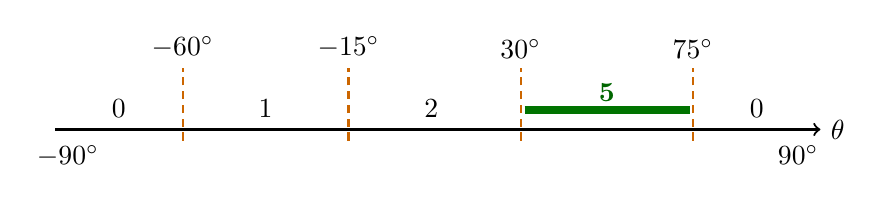
\begin{tikzpicture}[x=.81cm,y=.65cm]
\draw[->,thick] (0,0)--(12,0) node[right] {\(\theta\)};
\foreach \xx/\aa in {2/{-60^\circ},4.6/{-15^\circ},7.3/{30^\circ},10/{75^\circ}} {
\draw[densely dashed,orange!80!black,thick] (\xx,-.22)--(\xx,1.2);
\node[above] at (\xx,1.2) {\(\aa\)};
}
\draw[line width=3pt,green!45!black] (7.36,.38)--(9.96,.38);
\node at (1,.4) {0}; \node at (3.3,.4) {1}; \node at (5.9,.4) {2};
\node[green!40!black] at (8.65,.73) {\(\mathbf{5}\)};
\node at (11,.4) {0};
\node[below] at (.2,-.13) {\(-90^\circ\)};
\node[below] at (11.65,-.13) {\(90^\circ\)};
\end{tikzpicture}
\caption{An illustrative path for four unit vectors with polar angles \(30^\circ,75^\circ,120^\circ,165^\circ\), and edge weights \(w_{12}=w_{13}=w_{23}=w_{24}=1\), \(w_{14}=-1\), \(w_{34}=5\). The five interval scores are \(0,1,2,5,0\). This arbitrary embedding is not a solved SDP.}
\label{fig:toy}
\end{figure}

\section{Repeated arcs and tangent proposals}
For \(p>2\), infinitely many unit \(u\perp r\) exist. The algorithm repeats \cref{alg:arc} for a finite budget \(T\), accepting a newly realized normal only if its cut strictly exceeds the incumbent. There are three proposal modes:
\begin{description}
\item[Random:] Draw \(z\sim N(0,I_p)\) and take \(u=[z-(z^\top r)r]/\|z-(z^\top r)r\|\), uniformly oriented in the tangent subspace.
\item[Gain-guided:] Compute signed one-flip gains \(\Delta_i\), select vertices where \(\Delta_i<-10^{-9}\), form a gain-weighted combination of their embedding vectors and orthogonally project it onto \(r^\perp\).
\item[Boundary-guided:] Select up to 96 vertices with smallest \(|\Delta_i|\), combine their vectors with independent random signs, and project onto \(r^\perp\).
\end{description}
These descriptions follow the implemented \texttt{eva\_direct\_rounding.py}, not an idealized intended heuristic. A \emph{negative} \(\Delta_i\) in \eqref{eq:gain} means a harmful single flip. The source comment describing gain guidance as targeting improving flips therefore does not match its negative-gain selection. Likewise, boundary guidance uses small \emph{absolute flip gain}, not the geometric margin \(|y_i^\top r|\). Both questions require targeted ablation before attributing improvement to their intended motivations.

\begin{proposition}[Monotonicity and termination of strict improvement]
If accepted normals are independently rescored and only strict improvements are retained, the incumbent cut never decreases. It can undergo at most \(2^{n-1}-1\) strict improvements.
\end{proposition}
\begin{proof}
Monotonicity follows by acceptance. Every strict improvement corresponds to a new bipartition, and complementary spins represent the same cut; at most \(2^{n-1}\) bipartitions exist.
\end{proof}
This is \emph{not} a guarantee of global best hyperplane or even adjacency-based local optimality. The objective \(F(r)\) is piecewise constant on the sphere, making ordinary gradient stationarity uninformative. In dimension \(p=2\), one complete semicircle enumerates all homogeneous linear cut partitions up to complementation; in higher dimensions, a finite collection of arcs generally does not.

\section{Inherited approximation guarantee}
Define \(W_-=\sum_{\{i,j\}\in E}\min(w_{ij},0)\le0\). For an optimal solution \(X^\star\) of the SDP with unit diagonal, uniform GW initialization, and pathwise retention of the original cut, the following signed extension holds. Mere primal feasibility of an arbitrary factor is insufficient to compare its objective with \(\mathrm{OPT}\).
\begin{proposition}[Shifted signed-GW bound]
If the returned cut is never worse than the uniformly rounded starting cut, then
\begin{equation}\label{eq:shift}
\mathbb E[\Ccut(x_{\rm out})-W_-]\ge
\alpha_{\rm GW}(\mathrm{OPT}-W_-),\qquad \alpha_{\rm GW}\simeq0.878567.
\end{equation}
\end{proposition}
\begin{proof}
For an edge angle \(\phi=\arccos(X_{ij})\), put \(q=(1-\cos\phi)/2\) and \(p=\phi/\pi\), the SDP cut fraction and GW separation probability. For all \(\phi\in[0,\pi]\), \(p\ge\alpha_{\rm GW}q\); applying this to \(\pi-\phi\) gives \(1-p\ge\alpha_{\rm GW}(1-q)\). The shifted objective is the sum of positive-weight contributions of \emph{cut} edges and absolute negative-weight contributions of \emph{uncut} edges. Taking expectations and applying both inequalities yields \(\mathbb E[\Ccut(x_{\rm GW})-W_-]\ge\alpha_{\rm GW}(\mathrm{SDP}(X^\star)-W_-)\ge\alpha_{\rm GW}(\mathrm{OPT}-W_-)\). Pathwise retention transfers the bound to the returned cut.
\end{proof}
An approximate low-rank EVA factor without a certified SDP-optimality relation does not automatically justify a formal approximation bound against \(\mathrm{OPT}\). Adaptive tangent directions need not be uniform, and monotone improvement does not strengthen \(\alpha_{\rm GW}\).

\section{Experiment025: preliminary results and limits}
The repository reports completion of 71 G-set graphs, 18 initializer methods and 16 paired GW starting directions per graph-method cell: 20,448 saved seed checkpoints \citep{maxkcutrepo}. Each seed underwent the common full refinement of up to 20 positive-flip sweeps, 30 KL passes and 80 ILS cycles. The best \emph{ever observed} signed cut across those iterations and 16 starts is the method's value. No original EVA factor or SDP was recomputed for this paper. The available analysis is based on a compact 1,278-row graph-method summary; the full saved partitions have not been independently audited or verified backed up outside the university VM.

For graph \(g\), method \(m\), let \(C_{gm}\) be its best of 16 \emph{after common refinement}, with \(C_{g0}\) the similarly refined GW baseline. The reported equally weighted average relative gain is
\begin{equation}\label{eq:measure}
R_m=\frac{100}{71}\sum_{g=1}^{71}\frac{C_{gm}-C_{g0}}{C_{g0}}.
\end{equation}
All archived baseline values are positive. Intervals come from 30,000 percentile graph-level bootstrap resamples with seed 20261103, not from independently verified per-seed inference.

\begin{table}[t]
\centering\small
\caption{Provisional best-of-16, post-refinement comparisons with GW-RR. Intervals are graph-bootstrap 95\% percentiles; W/T/L counts graphs won/tied/lost against the refined GW baseline.}
\label{tab:results}
\begin{tabular}{lrrr}
\toprule
Method & Mean gain (\%) & 95\% interval (\%) & W/T/L\\
\midrule
Hyperplane Sweep & \(\mathbf{+0.3176}\) & [0.2252,0.4196] & 59/7/5\\
Paired-control & +0.2719 & [0.1782,0.3729] & 55/8/8\\
EM--Gibbs & +0.2707 & [0.1956,0.3522] & 59/9/3\\
Cut-aware \(k\)-means & +0.2668 & [0.1775,0.3631] & 56/5/10\\
EM--Hard & +0.2582 & [0.1839,0.3392] & 58/9/4\\
GW-RR & 0 & [0,0] & 0/71/0\\
\bottomrule
\end{tabular}
\end{table}
Hyperplane Sweep is the observed leader for the chosen equal-graph best-of-16 measure, but it does \emph{not} significantly dominate the four closest competitors under the report's graph-level two-sided signed-rank tests of \emph{absolute cut differences} (reported \(p=0.226,0.163,0.110,0.0828\)). These tests target a different estimand from bootstrap intervals on mean \emph{relative} improvements.

\begin{table}[t]
\centering\small
\caption{Provisional Hyperplane Sweep mean relative best-of-16 gain by topology and sign category.}
\label{tab:family}
\begin{tabular}{lrr@{\qquad}lrr}
\toprule
Topology & Graphs & Gain (\%) & Edge weights & Graphs & Gain (\%)\\
\midrule
Random & 30 & +0.375 & Positive & 35 & +0.163\\
Planar & 24 & +0.411 & Signed & 36 & +0.468\\
Toroidal & 17 & +0.084 & & &\\
\bottomrule
\end{tabular}
\end{table}
These strata are exploratory and can be confounded. Another method, control-tabu, ranks higher within the random graph stratum. The in-sample graphwise 18-method oracle is not a deployable selection policy. The aggregate source also contains several method pairs with identical score profiles.

\paragraph{Scientific limits.}
The measurement combines raw initialization and later Flip/KL/ILS refinement; it does not identify the \emph{isolated} gain attributable to the sweep. Per-seed covariance, detailed stage trajectories and archived best partitions are unavailable in the aggregate input, so raw paired-seed inference and original-edge audits cannot be performed from these data alone. Reported wall seconds measure the last invocation rather than total compute, precluding fair cut-per-second comparisons. Previously listed feasible reference cuts are not certificates of true optima; we assert no newly verified benchmark records.

\section{Related work and decisive next experiments}
The mechanism differs from \citet{lang2004}, which searches \emph{offset thresholds} along a fixed direction, while we rotate the normal of a homogeneous separator. It also differs from geometrically altering SDP vectors \citep{zwick1999,feige2006}, clustering them \citep{rodriguez2020}, iterated SDPs \citep{felzenszwalb2022}, and reinforcement-learning normal selection \citep{maliakal2025}. The finite-event approach is a specific construction, but claims of novel combination require a systematic review of earlier event sweeps and directional local-search methods.

The highest-priority next experiment should reuse the saved EVA embeddings: independently rescore every retained best partition against original signed edges; publish a compact 20,448-row matched-seed stage table; compare random-only, negative-gain, positive-gain, small-absolute-gain, geometric-margin and hybrid tangent selectors; and report matched raw, post-flip, post-KL and post-ILS results under equal candidate-evaluation and CPU-time budgets. Validate exact path optimality separately using small, low-dimensional exhaustive hyperplane-cell enumeration.

\section{Conclusion}
A great-semicircle event sweep optimizes the exact signed cut among partitions realized along one normal-rotation path with a sorting-and-gain-update algorithm. The repeated method can improve GW rounding while retaining its original observed cut. The provisional Experiment025 ranking motivates further study but does not yet establish independent numerical verification, an equal-compute advantage or an improved approximation factor.

\section*{Reproducibility and status}
Source implementation: \url{https://github.com/heri-espino/maxkcut/blob/main/src/maxkcut/eva_direct_rounding.py}. Source aggregate and methodology: provisional draft PR \#75, \url{https://github.com/heri-espino/maxkcut/pull/75}; input aggregate SHA-256: \texttt{8a9d84cfc35f1d424519b862676facc288a6366bc1820e52975a2bf76678de6c}. This is a research manuscript, not a peer-reviewed publication or an audited benchmark-record announcement.

\bibliographystyle{plainnat}
\bibliography{references}
\end{document}
